%% Преамбула TeX-файла

% 1. Стиль и язык
\documentclass[utf8x, 12pt]{G7-32a} % Стиль (по умолчанию будет 14pt)

% Остальные стандартные настройки убраны в preamble-std.tex
\sloppy

% 1. Настройки стиля ГОСТ 7-32
% Для начала определяем, хотим мы или нет, чтобы рисунки и таблицы нумеровались в пределах раздела, или нам нужна сквозная нумерация.
% А не забыл ли автор букву 't' ?
\EqInChapter % формулы будут нумероваться в пределах раздела
\TableInChapter % таблицы будут нумероваться в пределах раздела
\PicInChapter % рисунки будут нумероваться в пределах раздела

% 2. Добавляем гипертекстовое оглавление в PDF
\usepackage[
bookmarks=true, colorlinks=true, unicode=true,
urlcolor=black,linkcolor=black, anchorcolor=black,
citecolor=black, menucolor=black, filecolor=black,
]{hyperref}

% 3. Изменение начертания шрифта --- после чего выглядит таймсоподобно.
% apt-get install scalable-cyrfonts-tex

\IfFileExists{cyrtimes.sty}
    {
        \usepackage{cyrtimespatched}
    }
    {
        % А если Times нету, то будет CM...
    }


% 4. Прочие полезные пакеты.
\usepackage{underscore} % Ура! Теперь можно писать подчёркивание.
                        % И нельзя использовать подчёркивание в файлах.
                        % Выбирай, но осторожно.

\usepackage{graphicx}   % Пакет для включения рисунков

 % 5. Любимые команды
\newcommand{\Code}[1]{\textbf{#1}}

% 6. Поля
% С такими оно полями оно работает по-умолчанию:
% \RequirePackage[left=20mm,right=10mm,top=20mm,bottom=20mm,headsep=0pt]{geometry}
% Если вас тошнит от поля в 10мм --- увеличивайте до 20-ти, ну и про переплёт не забывайте:


% Размер страницы
\usepackage{geometry}
%\geometry{paperheight=20cm}
%\geometry{paperwidth=15cm}

\geometry{right=20mm}
\geometry{left=20mm}
\geometry{top=8mm}
\geometry{bottom=15mm}

% 7. Tikz
\usepackage{tikz}
\usetikzlibrary{arrows,positioning,shadows}

% 8 Листинги

\usepackage{listings}

% Значения по умолчанию
\lstset{
  basicstyle= \footnotesize,
  breakatwhitespace=true,% разрыв строк только на whitespacce
  breaklines=true,       % переносить длинные строки
%   captionpos=b,          % подписи снизу -- вроде не надо
  inputencoding=koi8-r,
  numbers=left,          % нумерация слева
  numberstyle=\footnotesize,
  showspaces=false,      % показывать пробелы подчеркиваниями -- идиотизм 70-х годов
  showstringspaces=false,
  showtabs=false,        % и табы тоже
  stepnumber=1,
  tabsize=4,              % кому нужны табы по 8 символов?
  frame=single
}

% Стиль для псевдокода: строчки обычно короткие, поэтому размер шрифта побольше
\lstdefinestyle{pseudocode}{
  basicstyle=\small,
  keywordstyle=\color{black}\bfseries\underbar,
  language=Pseudocode,
  numberstyle=\footnotesize,
  commentstyle=\footnotesize\it
}

% Стиль для обычного кода: маленький шрифт
\lstdefinestyle{realcode}{
  basicstyle=\scriptsize,
  numberstyle=\footnotesize
}

% Стиль для коротких кусков обычного кода: средний шрифт
\lstdefinestyle{simplecode}{
  basicstyle=\footnotesize,
  numberstyle=\footnotesize
}

% Стиль для BNF
\lstdefinestyle{grammar}{
  basicstyle=\footnotesize,
  numberstyle=\footnotesize,
  stringstyle=\bfseries\ttfamily,
  language=BNF
}

% Определим свой язык для написания псевдокодов на основе Python
\lstdefinelanguage[]{Pseudocode}[]{Python}{
  morekeywords={each,empty,wait,do},% ключевые слова добавлять сюда
  morecomment=[s]{\{}{\}},% комменты {а-ля Pascal} смотрятся нагляднее
  literate=% а сюда добавлять операторы, которые хотите отображать как мат. символы
    {->}{\ensuremath{$\rightarrow$}~}2%
    {<-}{\ensuremath{$\leftarrow$}~}2%
    {:=}{\ensuremath{$\leftarrow$}~}2%
    {<--}{\ensuremath{$\Longleftarrow$}~}2%
}[keywords,comments]

% Свой язык для задания грамматик в BNF
\lstdefinelanguage[]{BNF}[]{}{
  morekeywords={},
  morecomment=[s]{@}{@},
  morestring=[b]",%
  literate=%
    {->}{\ensuremath{$\rightarrow$}~}2%
    {*}{\ensuremath{$^*$}~}2%
    {+}{\ensuremath{$^+$}~}2%
    {|}{\ensuremath{$|$}~}2%
}[keywords,comments,strings]

% Подписи к листингам на русском языке.
\renewcommand*\thelstnumber{\oldstylenums{\the\value{lstnumber}}}
\renewcommand\lstlistingname{\cyr\CYRL\cyri\cyrs\cyrt\cyri\cyrn\cyrg}
\renewcommand\lstlistlistingname{\cyr\CYRL\cyri\cyrs\cyrt\cyri\cyrn\cyrg\cyri}

% Произвольная нумерация списков.
\usepackage{enumerate}

% Вставлять pdf-страницы
\usepackage{pdfpages}

\usepackage{fancyhdr}

\usepackage{multicol}


\raggedbottom
\captionsetup[figure]{belowskip=0pt,aboveskip=0pt}
\setlength{\intextsep}{3pt plus 0pt minus 0pt}

%\usepackage{sidecap}
%\usepackage{floatrow}

\usepackage{setspace}



%\usepackage[perpage,para,symbol*]{footmisc}




\begin{document}



\frontmatter % выключает нумерацию ВСЕГО; здесь начинаются ненумерованные главы: реферат, введение, глоссарий, сокращения и прочее

% Команды \breakingbeforechapters и \nonbreakingbeforechapters
% управляют разрывом страницы перед главами.
% По-умолчанию страница разрывается.

% \nobreakingbeforechapters
% \breakingbeforechapters
\thispagestyle{empty} 
\newgeometry{left=5mm, right=5mm, top=2mm, bottom=0mm}

\begin{figure}[h!]
    \caption{Один из первопоселенцев Дома Варзар Дмитрий Васильевич преподавал математику в специальной школе при КГБ. Репрессирован в 1934 году. Расстрелян в 1937 году. Реабиллитирован в 1956 году <<за отсутствием состава преступления>>.}
    \begin{minipage}[h!]{40mm}
         \vspace{10pt}
         \begin{center}
         \vspace{-15pt}
         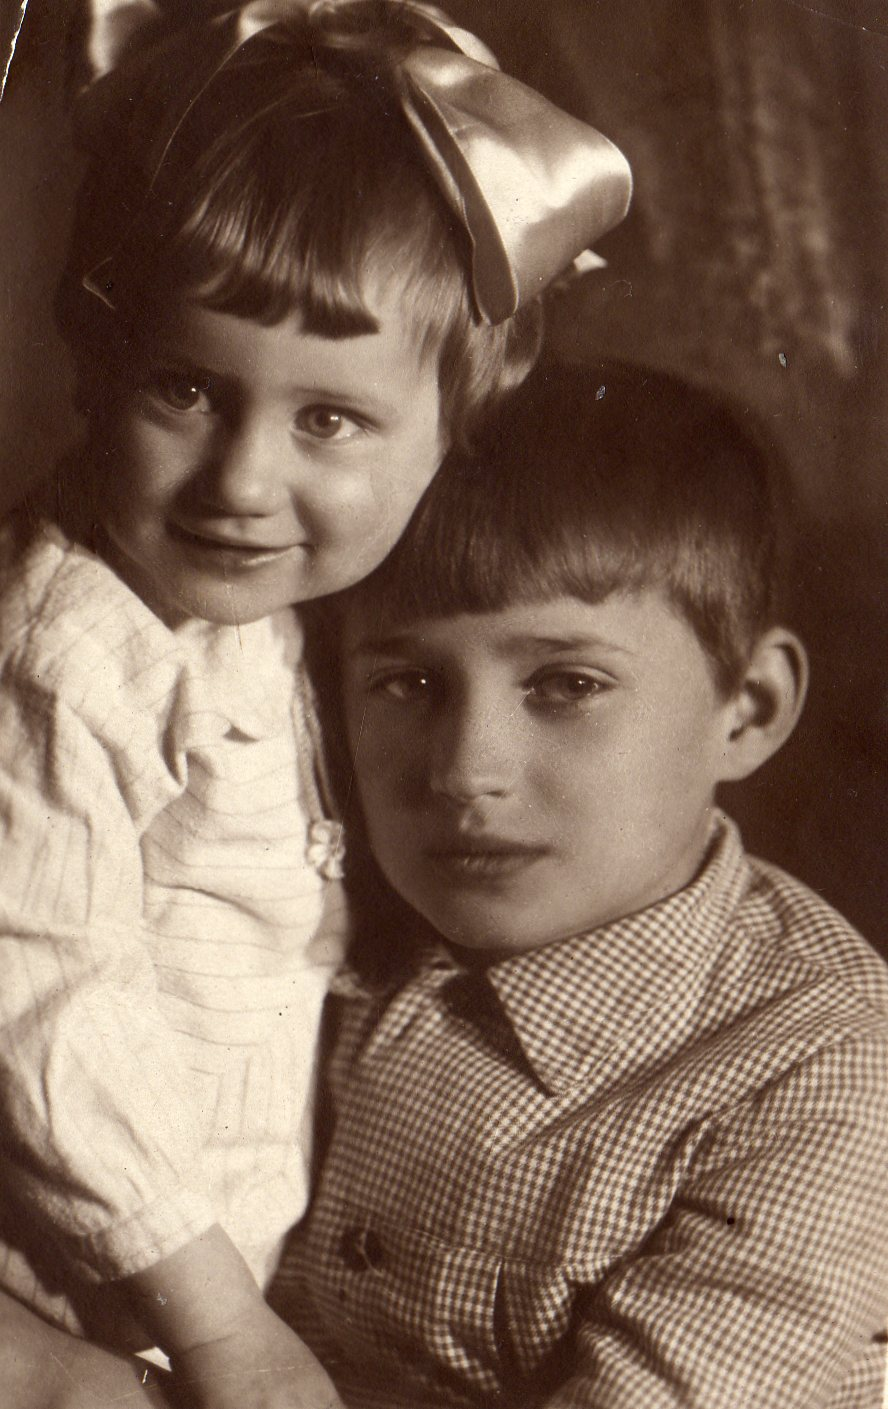
\includegraphics[height=40mm]{inc/Varzar/11.jpg} 
         \end{center}
         \vspace{-10pt}
         Ксения и Сева \\Варзар. 1934 г.
    \end{minipage}
    \hfill
   \begin{minipage}[h]{55mm}
       \begin{center}
       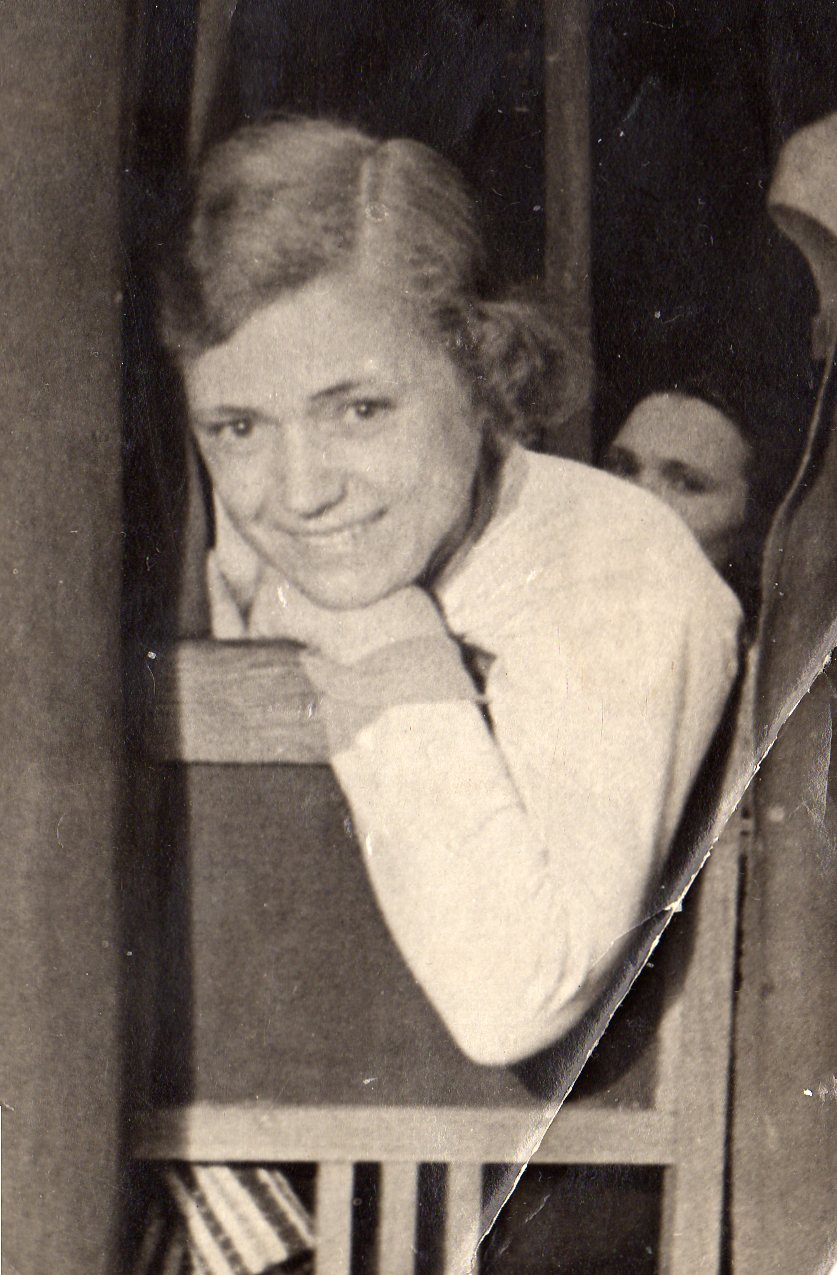
\includegraphics[height=50mm]{inc/Varzar/12.jpg} 
       \end{center}
       \caption{Наша мама~-- Варзар Евдокия Ивановна. Статистик. 1940 г.}
   \end{minipage}
   \hfill
    \begin{minipage}[h!]{55mm}
        \begin{center}
        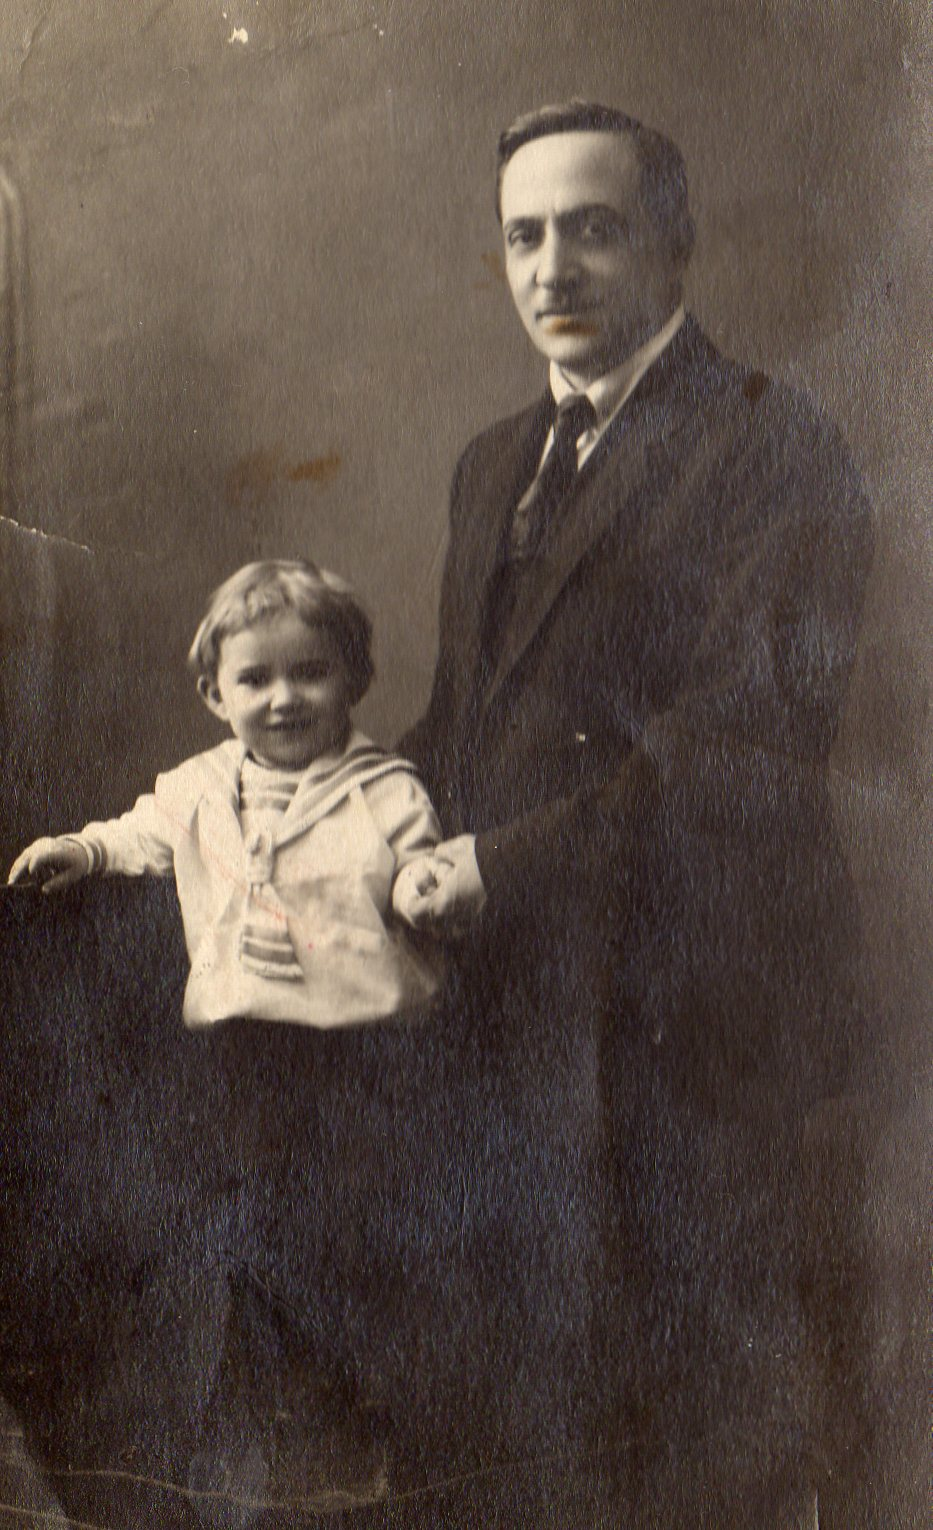
\includegraphics[height=50mm]{inc/Varzar/13.jpg}
        \end{center}
        \caption{Наша папа~-- Варзар Дмитрий Васильевич с сыном. 1925 г.}
    \end{minipage}
    \hfill
    \begin{minipage}[h!]{40mm}
         \vspace{10pt}
        \begin{center}
        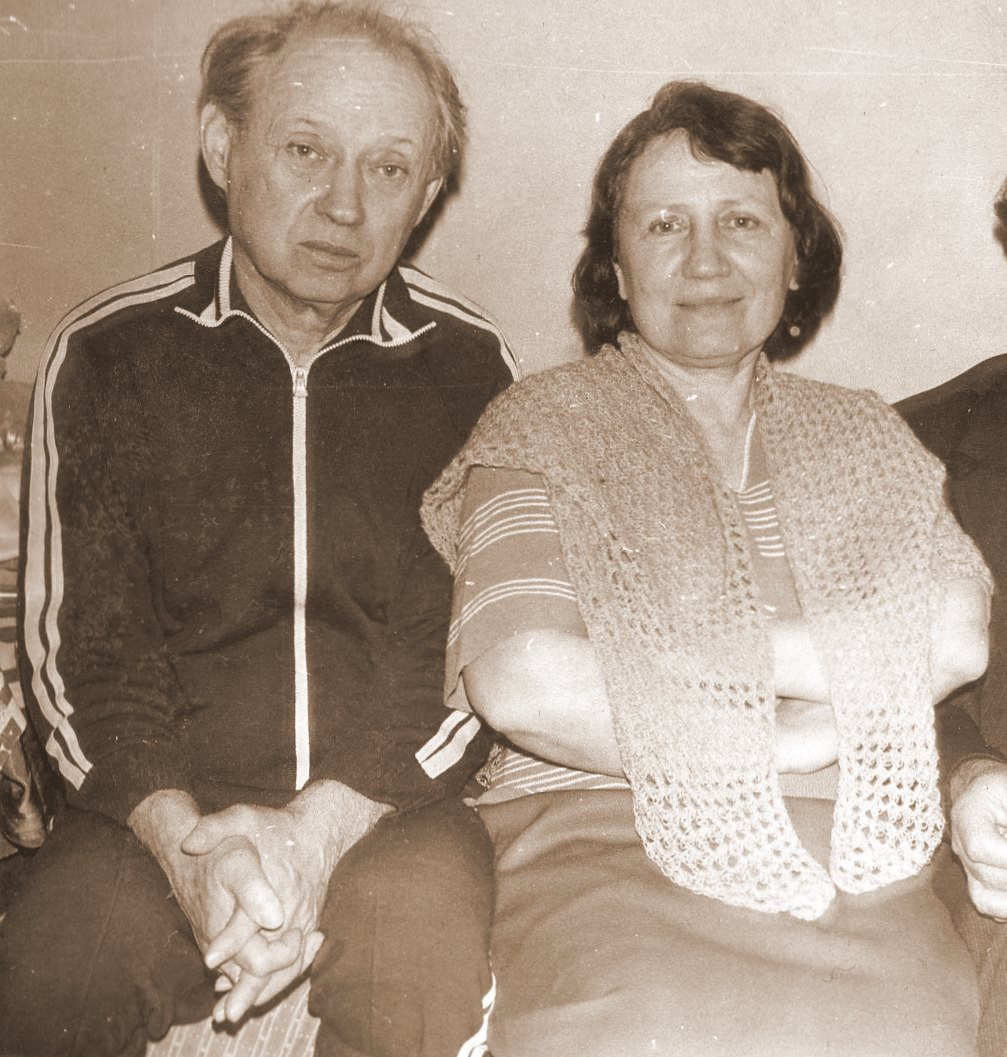
\includegraphics[height=40mm]{inc/Varzar/14.jpg}
        \end{center}
        \vspace{-10pt}
        \caption{Всеволод (Сева) и Ксения Варзар. \\1982 г.}
    \end{minipage}
\end{figure}
%\vfill
%vspace{5pt}

\begin{figure}[h!]
    \begin{minipage}[h!]{50mm}
         \vspace{10pt}
         \begin{center}
         \vspace{-15pt}
         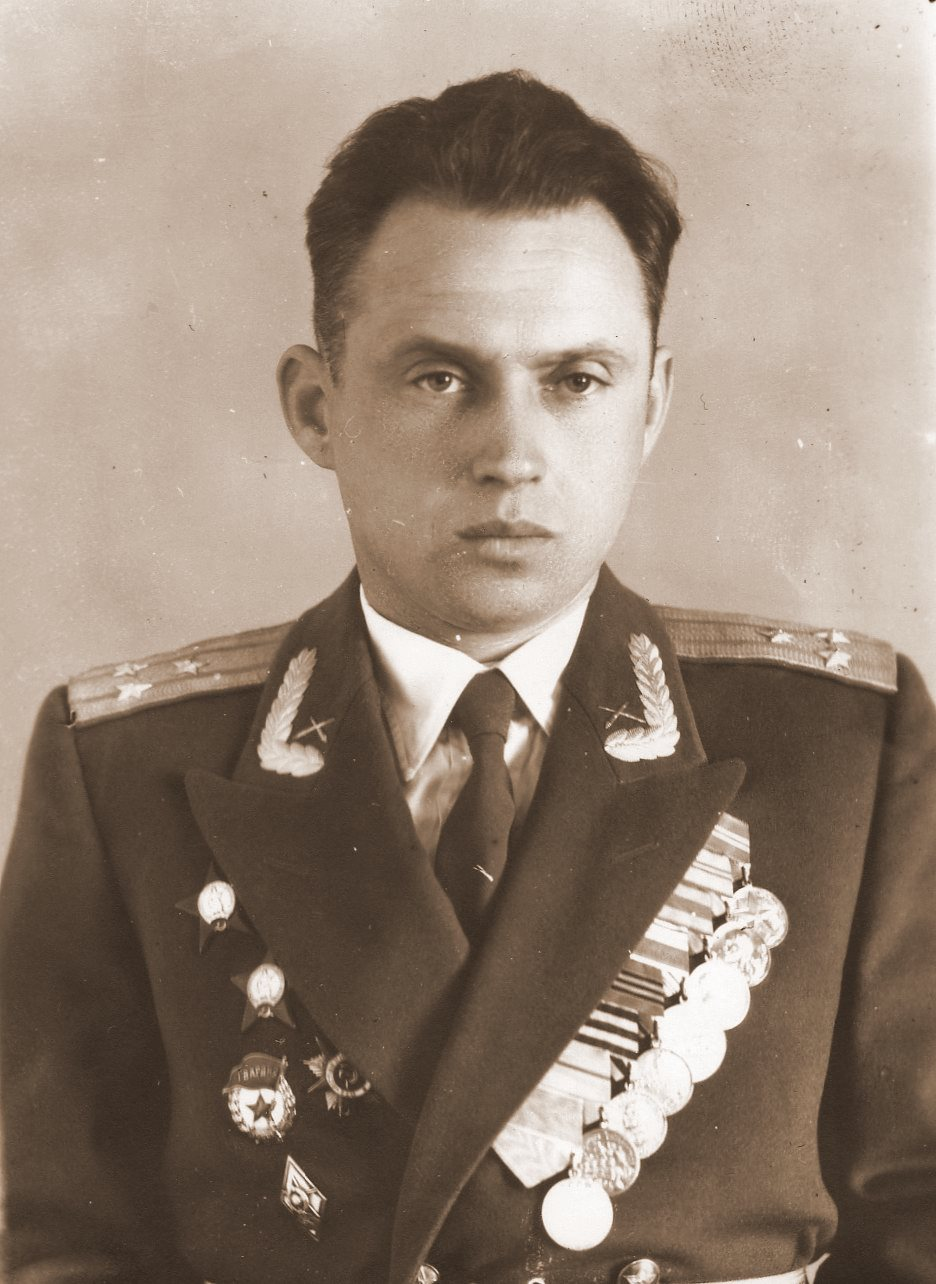
\includegraphics[height=45mm]{inc/Varzar/21.jpg} 
         \end{center}
         \vspace{-10pt}
         Сева. Инженер-артиллерист. Конец 50-х годов.
    \end{minipage}
    \hfill
   \begin{minipage}[h]{70mm}
       \begin{center}
       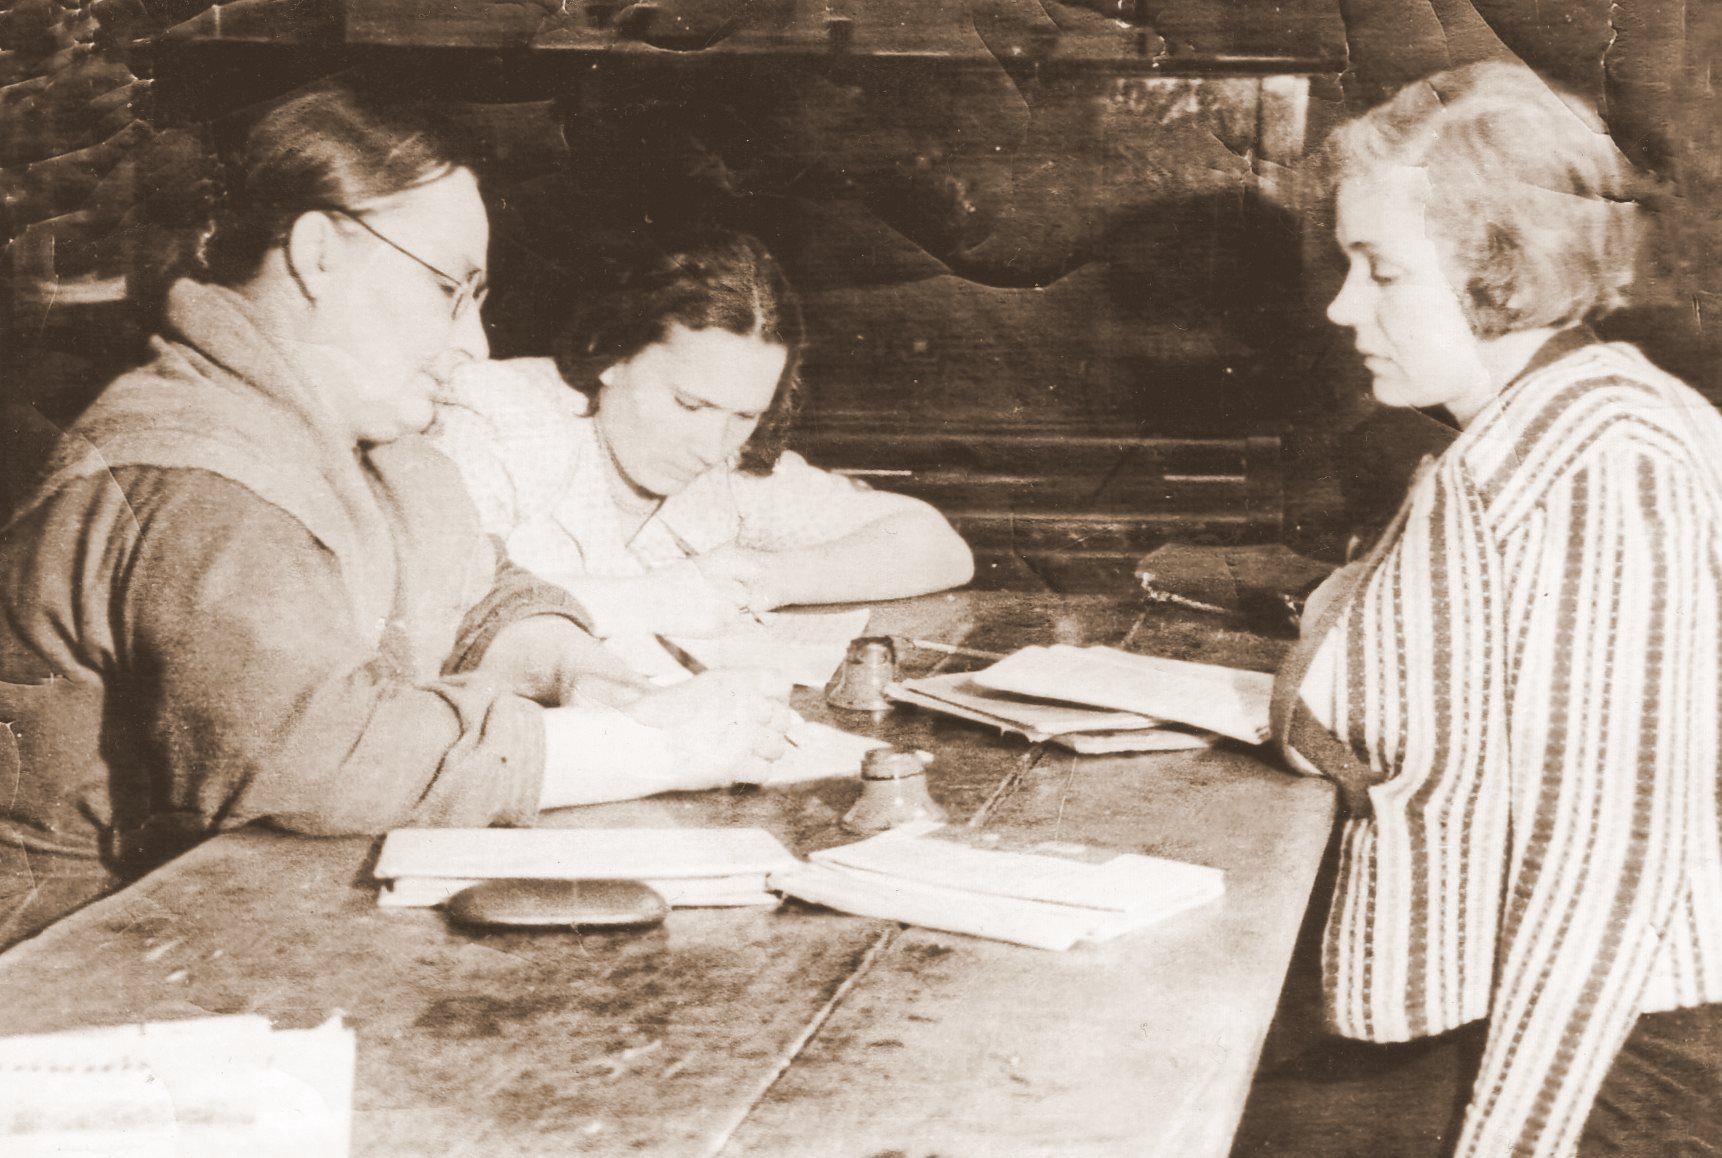
\includegraphics[height=45mm]{inc/Varzar/22.jpg} 
       \end{center}
       \caption{Евдокия Ивановна ведет занятия Ликбеза.}
   \end{minipage}
   \hfill
    \begin{minipage}[h!]{50mm}
        \begin{center}
        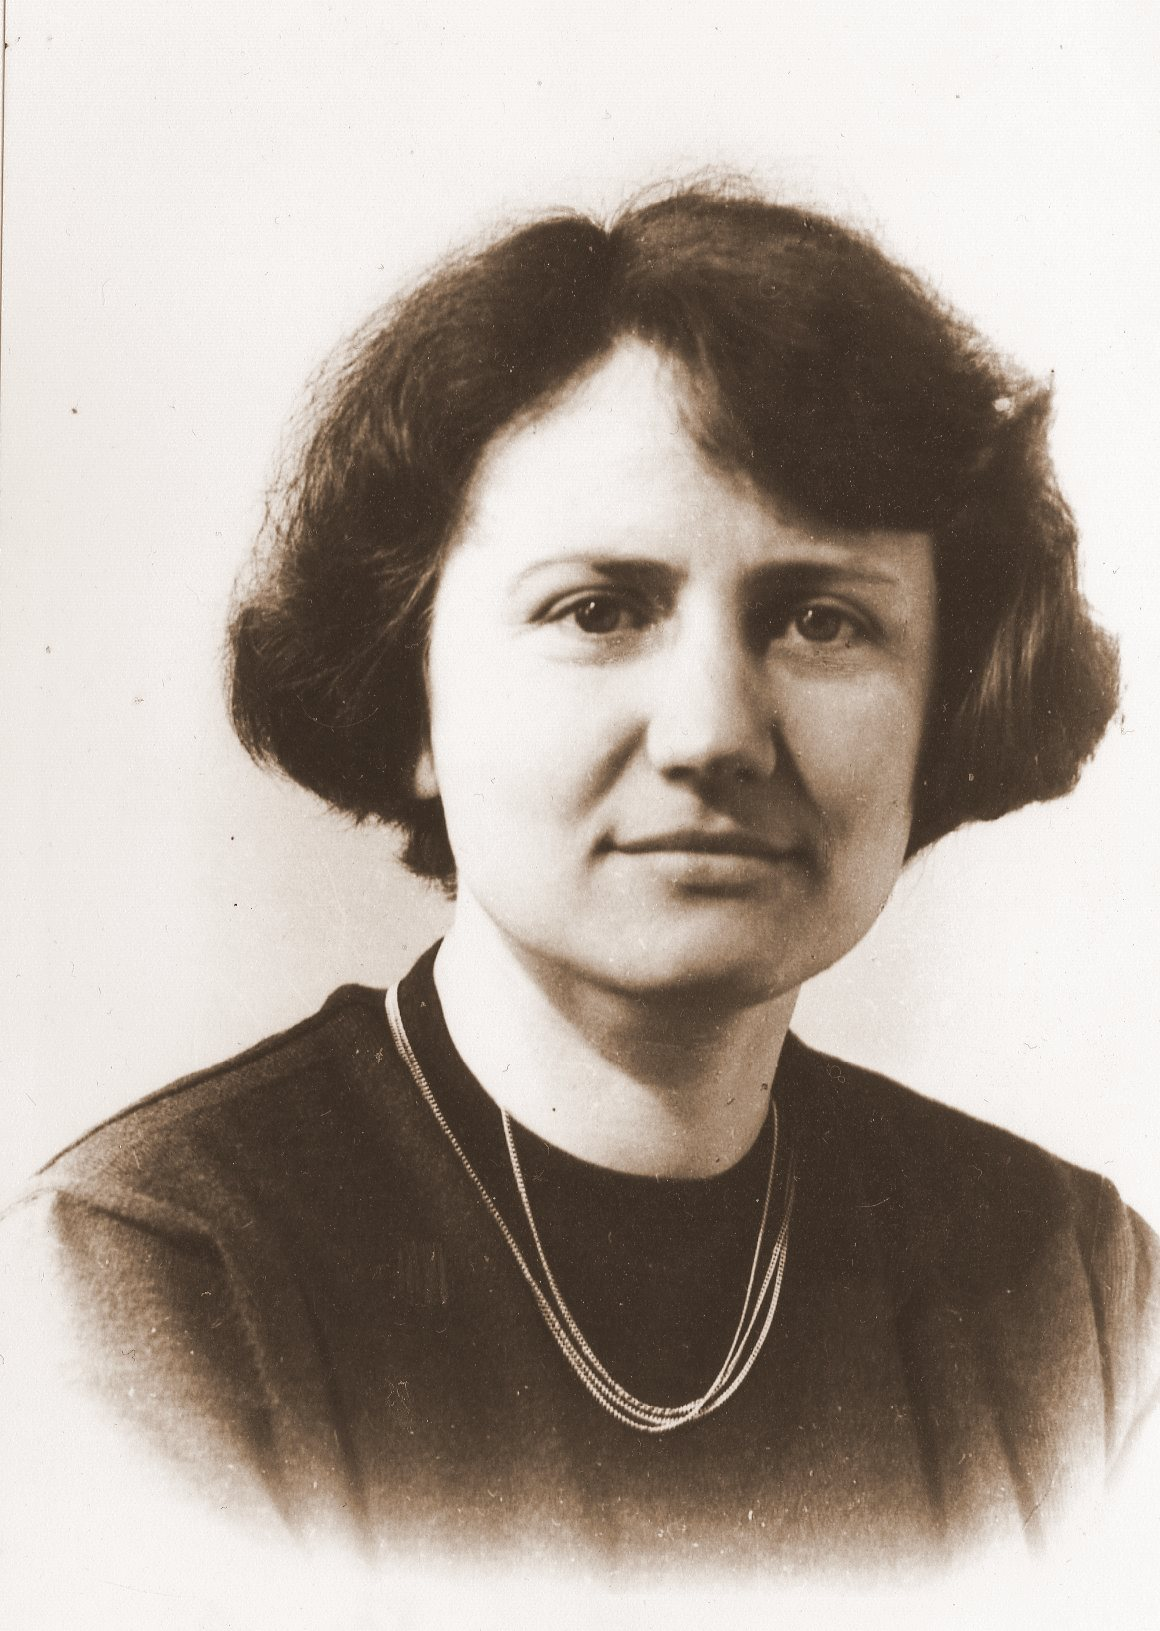
\includegraphics[height=45mm]{inc/Varzar/23.jpg}
        \end{center}
        \caption{Ксения. Инженер-геолог ГлавАПУ. Конец 50-х годов.}
    \end{minipage}
\end{figure}

\vspace{5pt}

\begin{figure}[h!]
    \begin{minipage}[h!]{61mm}
         \vspace{10pt}
         \begin{center}
         \vspace{-15pt}
         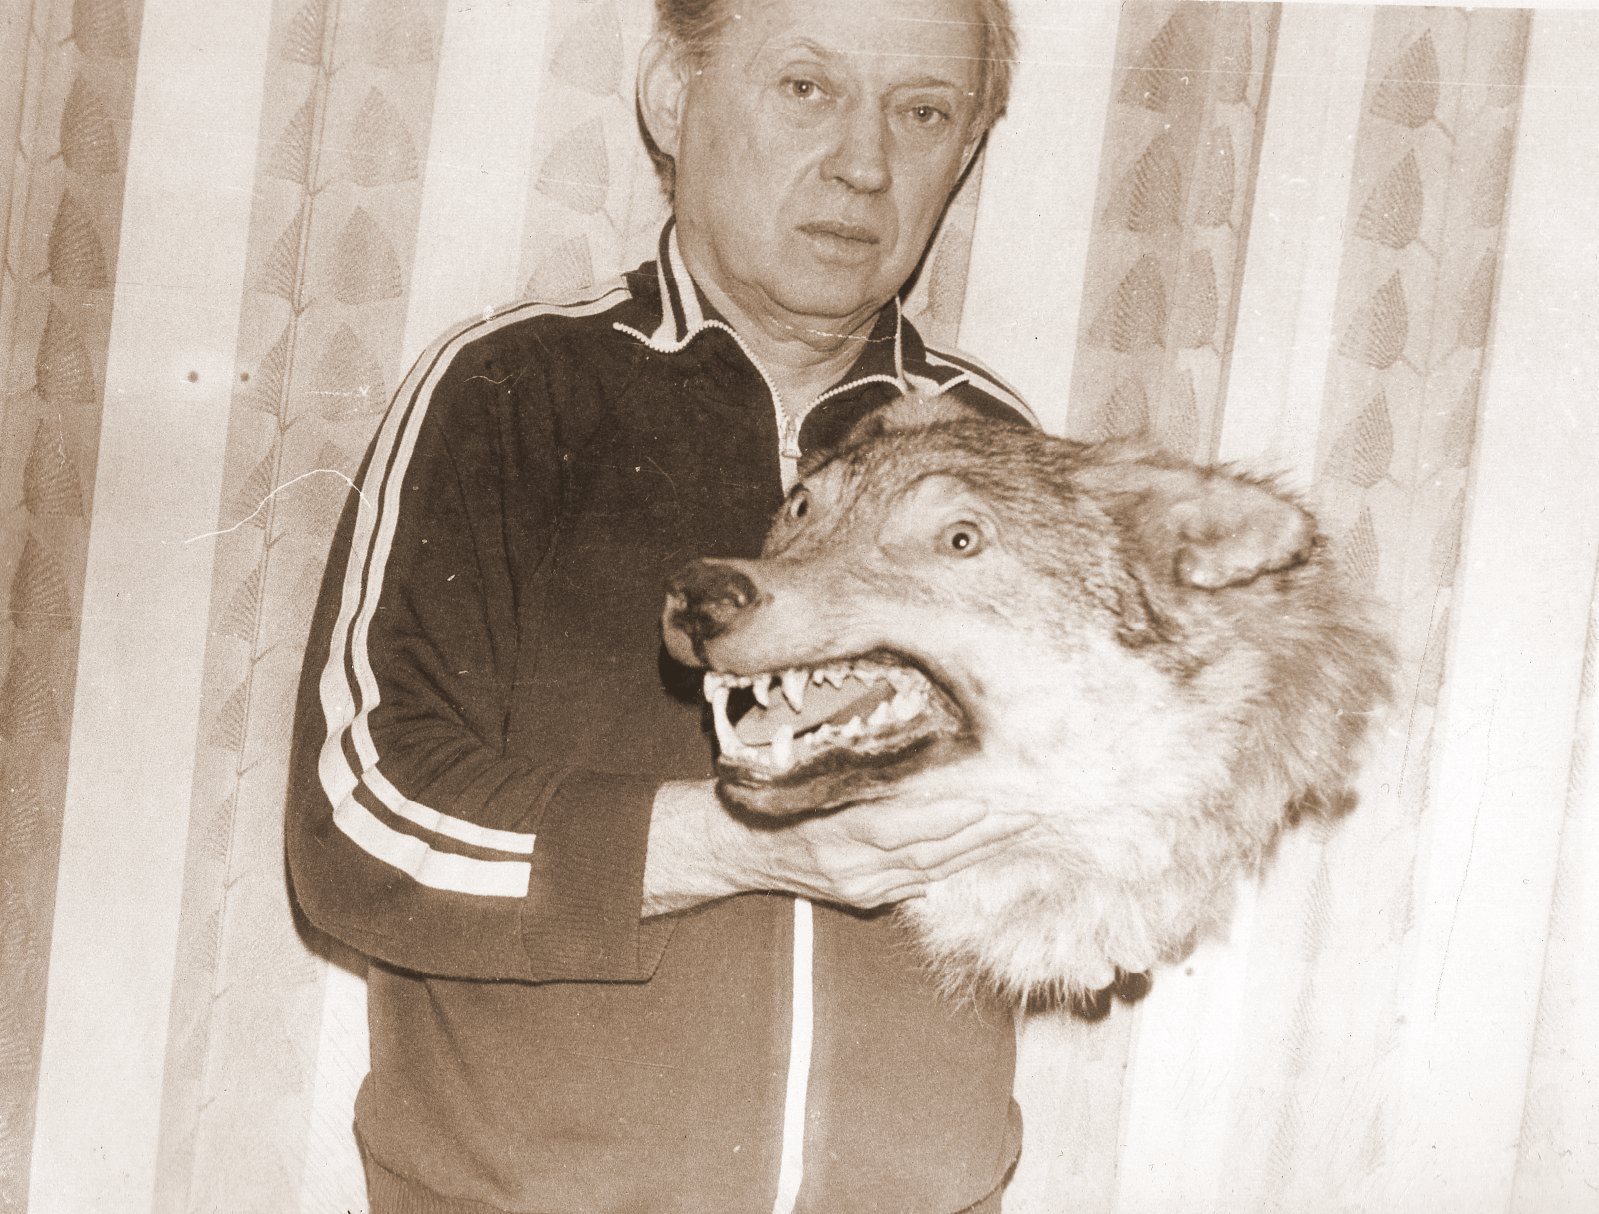
\includegraphics[width=61mm]{inc/Varzar/31.jpg} 
         \end{center}
         \vspace{-10pt}
         Сева охотник.
    \end{minipage}
    \hfill
   \begin{minipage}[h]{65mm}
       \begin{center}
       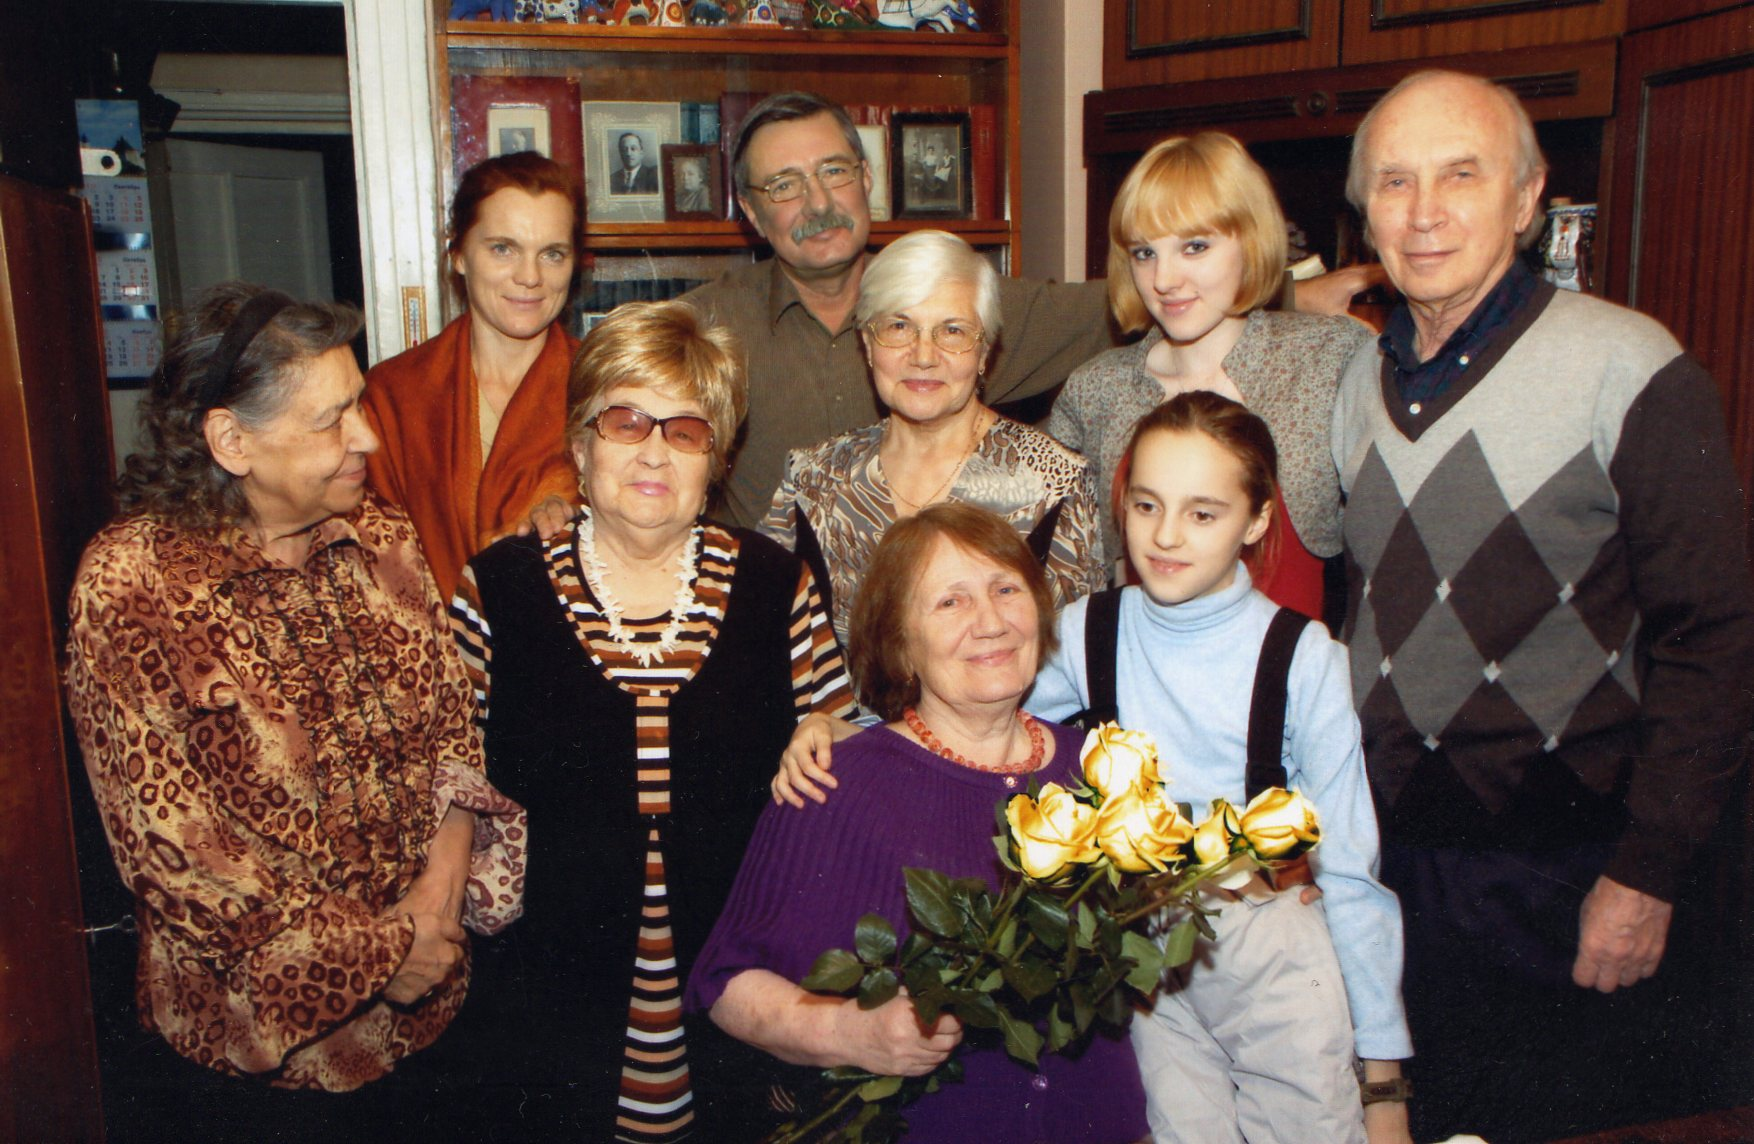
\includegraphics[width=70mm]{inc/Varzar/32.jpg} 
       \end{center}
       \caption{Юбилей Ксении.}
   \end{minipage}
   \hfill
    \begin{minipage}[h!]{32mm}
        \begin{center}
        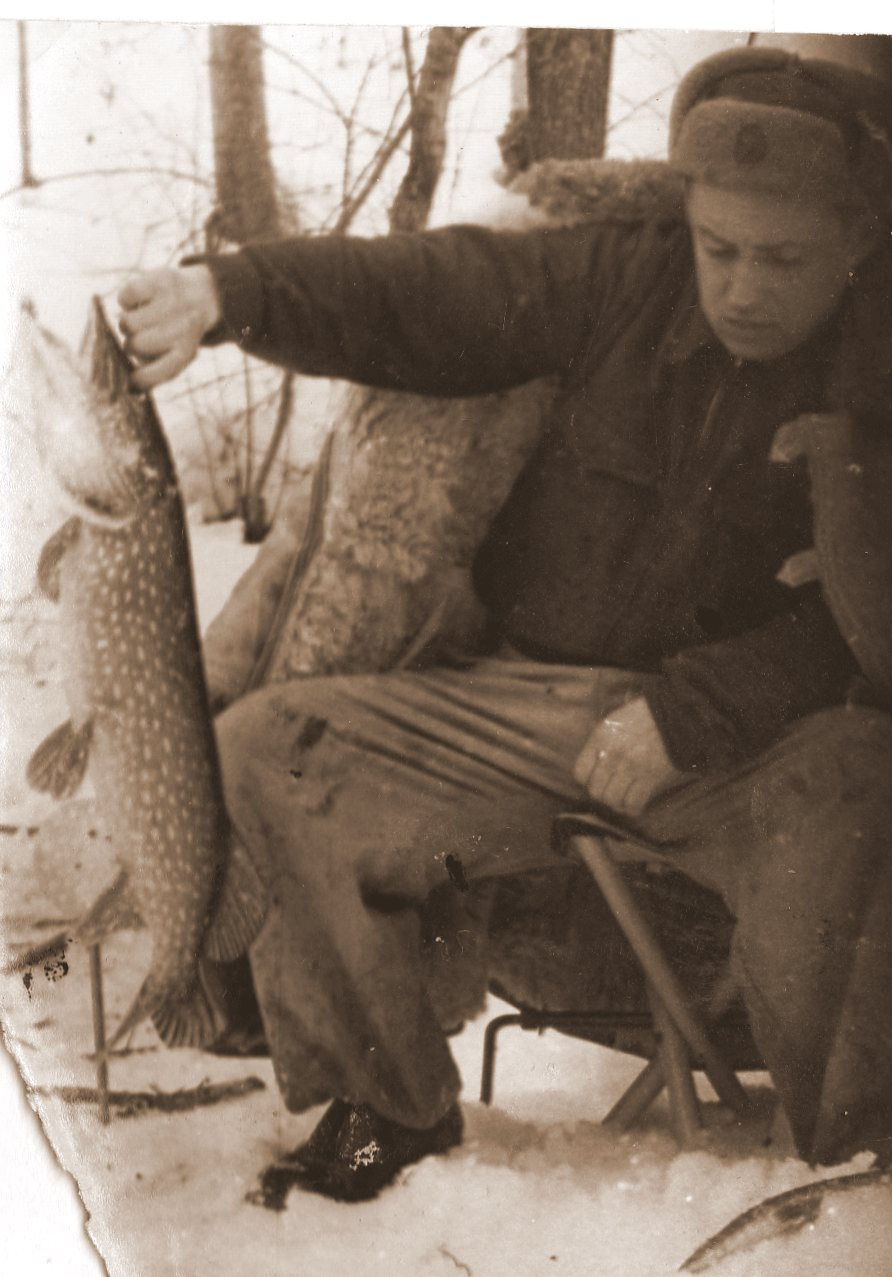
\includegraphics[width=32mm]{inc/Varzar/33.jpg}
        \end{center}
        \caption{Сева рыболов.}
    \end{minipage}
\end{figure}

\vspace{5pt}

\begin{figure}[h!]
    \begin{minipage}[h!]{45mm}
         \vspace{10pt}
         \begin{center}
         \vspace{-15pt}
         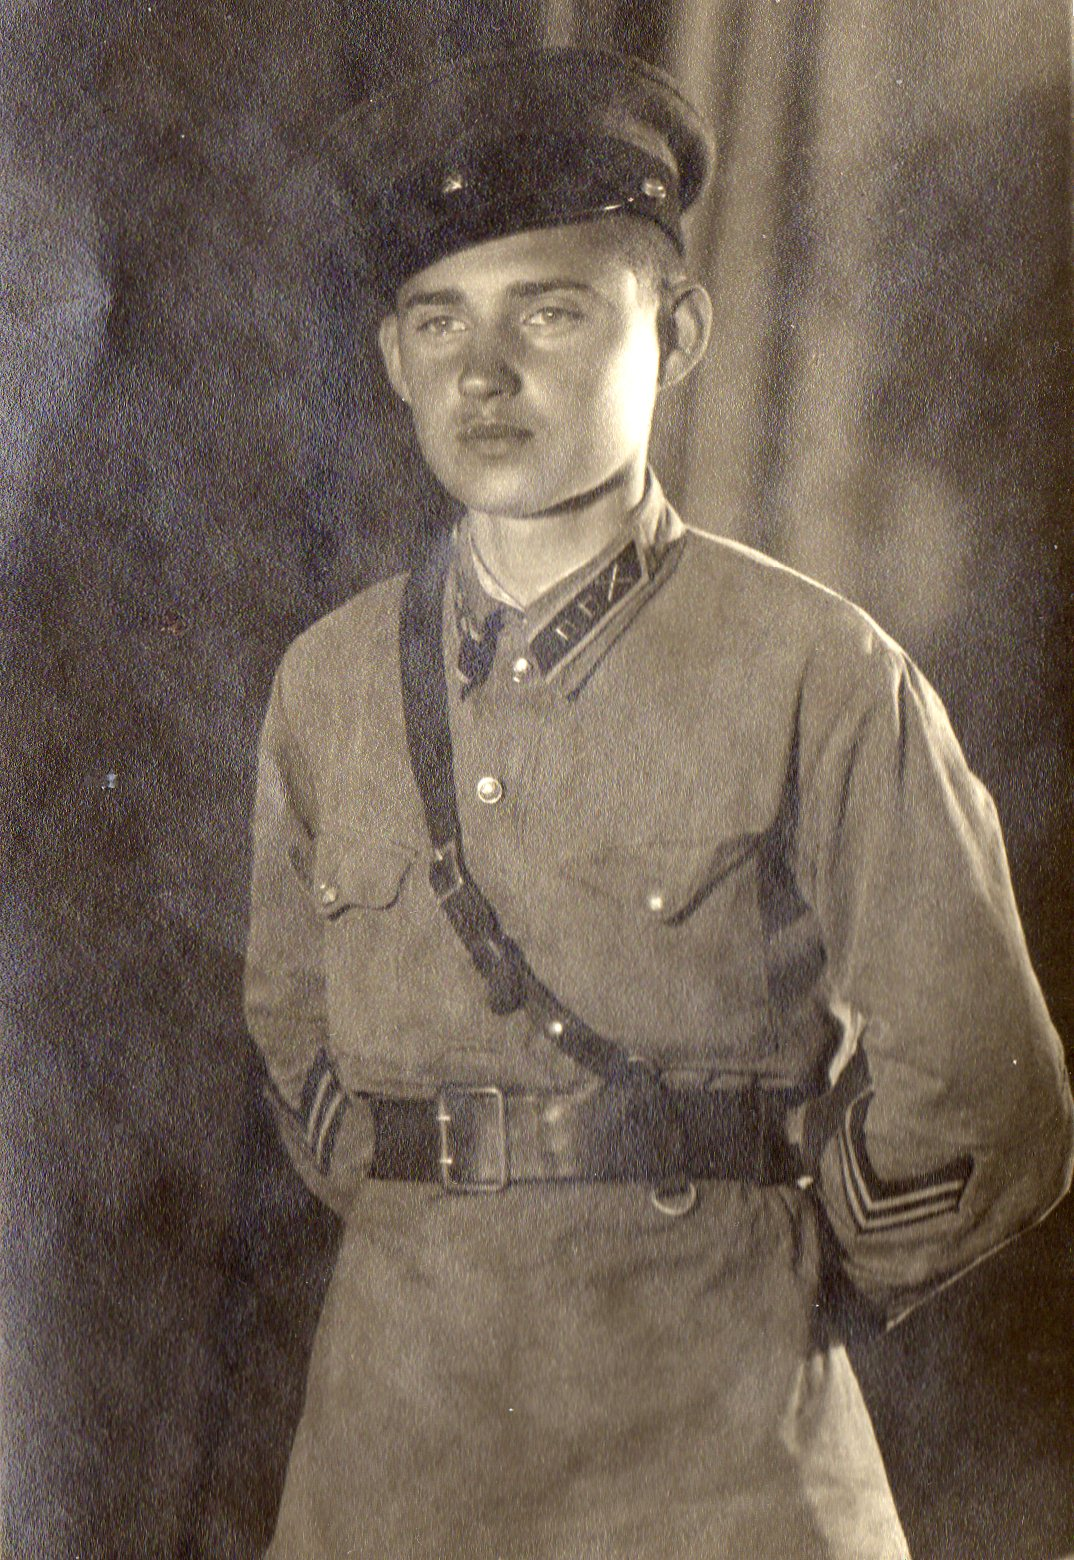
\includegraphics[height=50mm]{inc/Varzar/41.jpg} 
         \end{center}
         \vspace{-10pt}
    \end{minipage}
    \hfill
   \begin{minipage}[h]{65mm}
       \begin{center}
       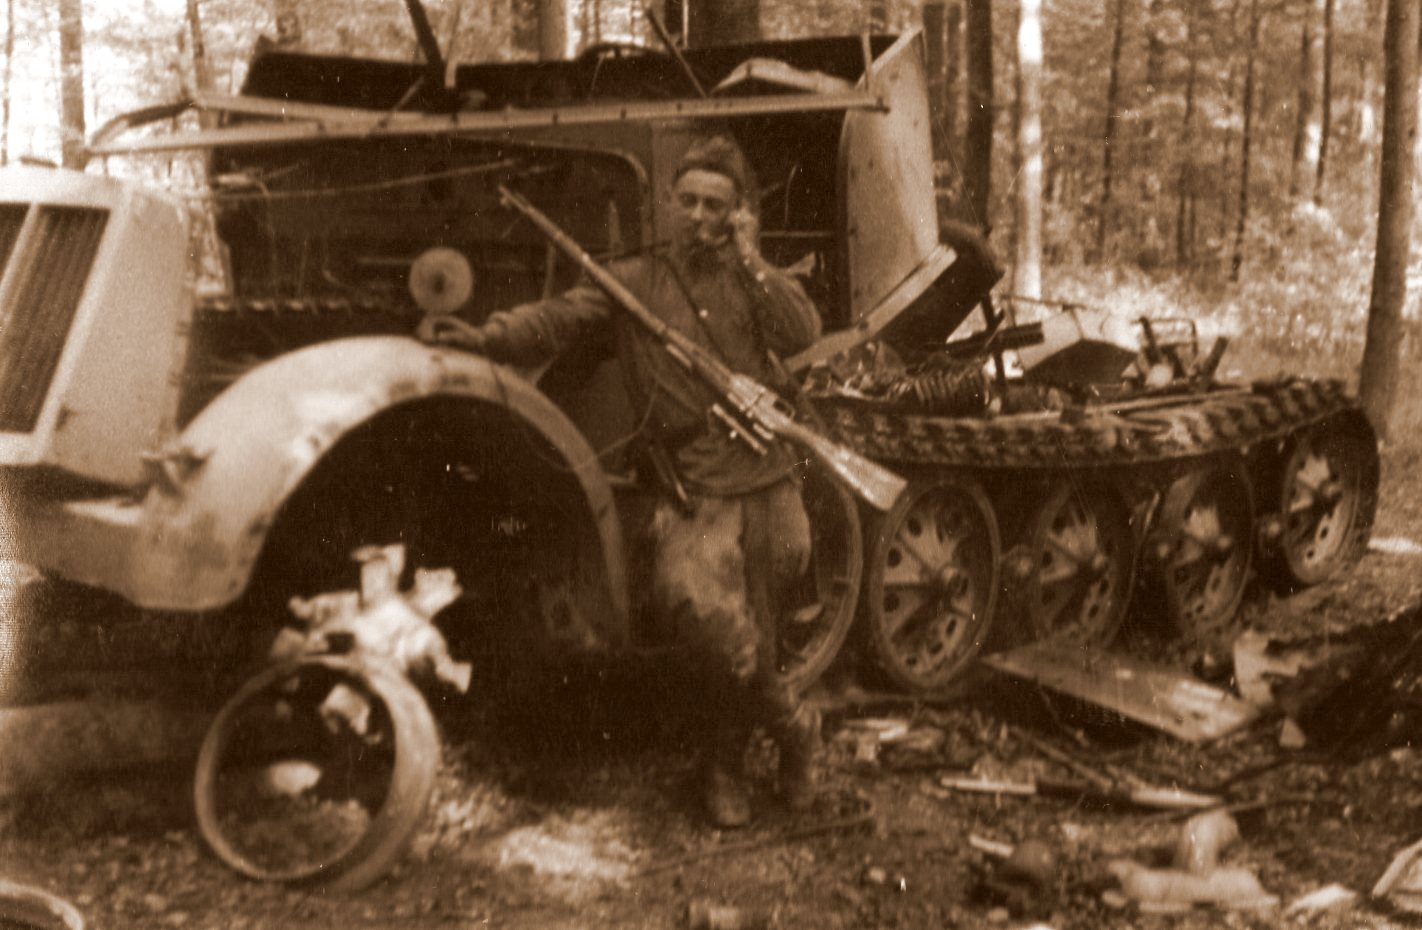
\includegraphics[height=50mm]{inc/Varzar/42.jpg} 
       \end{center}
   \end{minipage}
   \hfill
    \begin{minipage}[h!]{45mm}
        \begin{center}
        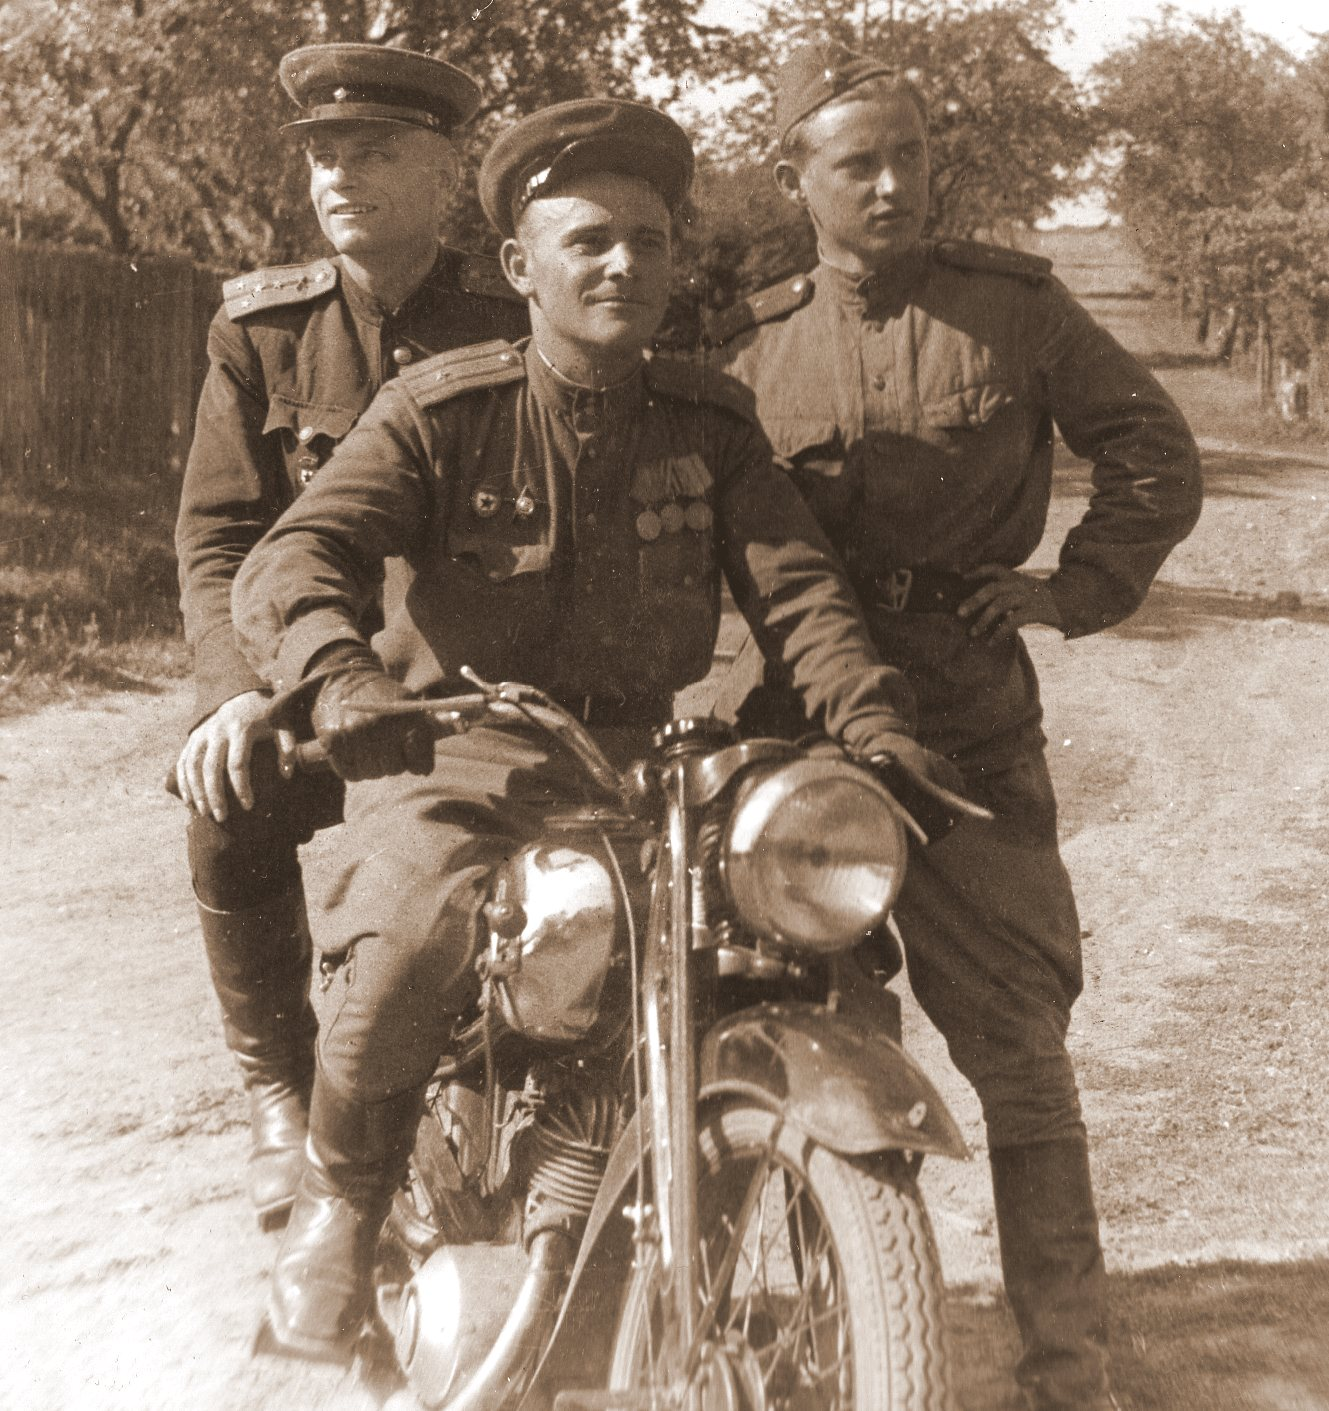
\includegraphics[height=50mm]{inc/Varzar/43a.jpg}
        \end{center}
    \end{minipage}
    \caption{На войне: от начала до конца.}
\end{figure}

\vspace{-20pt}


\mainmatter % это включает нумерацию глав и секций в документе ниже



\backmatter %% Здесь заканчивается нумерованная часть документа и начинаются ссылки и
            %% заключение



\appendix   % Тут идут приложения



\end{document}

%%% Local Variables:
%%% mode: latex
%%% TeX-master: t
%%% End:
